% ! TeX program = lualatex
\documentclass[a4paper,11pt]{article} 
% packages
\usepackage{censor}
\StopCensoring
\usepackage{fontspec}
\setmainfont{EB Garamond}
% for tironian et fallback
% % \directlua{luaotfload.add_fallback
% % ("emojifallback",
% %      {"Noto Serif:mode=harf"}
% % )}
% % \setmainfont{EB Garamond}[RawFeature={fallback=emojifallback}]

\setmonofont[Scale=MatchLowercase]{Deja Vu Sans Mono}
\usepackage[a4paper,left=2cm,right=2cm,top=\dimexpr15mm+1.5\baselineskip,bottom=2cm]{geometry}
\setlength{\parindent}{0pt}

\usepackage{fancyhdr}       % Headers and footers 
\fancyhead[R]{\normalfont \leftmark}
\fancyhead[L]{}
\pagestyle{fancy}

\usepackage{microtype}      % Slightly tweak font spacing for aesthetics
\usepackage[english]{babel} % Language hyphenation and typographical rules
\usepackage{xcolor}
\definecolor{linkblue}{RGB}{0, 64, 128}
\usepackage[final, colorlinks = false, urlcolor = linkblue]{hyperref} 
% \newcommand{\secref}[1]{\textbf{§~\nameref{#1}}}
\newcommand{\secref}[1]{\textbf{§\ref{#1}~\nameref{#1}}}

\usepackage{changepage}     % adjust margins on the fly
\usepackage{amsmath,amssymb}

\usepackage{minted}
\usemintedstyle{algol_nu}

\usepackage{pgfplots}
\pgfplotsset{width=\textwidth,compat=1.9}

\usepackage{caption}
\newenvironment{code}{\captionsetup{type=listing}}{}
\captionsetup[listing]{skip=0pt}
\setlength{\abovecaptionskip}{5pt}
\setlength{\belowcaptionskip}{5pt}

\usepackage[yyyymmdd]{datetime}
\renewcommand{\dateseparator}{--}

\usepackage{enumitem}

\usepackage{titlesec}

\author{Andrew Hayes}

\begin{document}
\begin{titlepage}
    \begin{center}
        \hrule
        \vspace*{0.6cm}
        \Huge \textsc{ct414}
        \vspace*{0.6cm}
        \hrule
        \LARGE
       \vspace{0.5cm}
       Distributed Systems \& Co-Operative Computing
       \vspace{0.5cm}
       \hrule

       \vfill

       \hrule
        \begin{minipage}{0.495\textwidth} 
            \vspace{0.4em}
            \raggedright
            \normalsize 
            \begin{tabular}{@{}l l}
                Name: & Andrew Hayes \\
                Student ID: & 21321503 \\
                E-mail: & \href{mailto://a.hayes18@universityofgalway.ie}{a.hayes18@universityofgalway.ie} \\
            \end{tabular}
        \end{minipage}
        \begin{minipage}{0.495\textwidth} 
            \raggedleft
            \vspace*{0.8cm}
            \Large
            \today
            \vspace*{0.6cm}
        \end{minipage}
        \medskip\hrule 
    \end{center}
\end{titlepage}

\pagenumbering{roman}
\newpage
\tableofcontents
\newpage
\setcounter{page}{1}
\pagenumbering{arabic}

\section{Introduction}
\subsection{Client-Server Architectures}
\subsubsection{Two-Tier Architectures}
A \textbf{two-tier client-server architecture} is a client-server architecture wherein a client talks directly to a server, with no intervening server.
It is typically used in small environments ($\lesssim$ 50 users).
\\\\
A common development error is to prototype an application in a small, two-tier environment, and then scale up by simply adding more users to the server:
this approach will usually result in an ineffective system, as the server becomes overwhelmed.
To properly scale to hundreds or thousands of users, it is usually necessary to move to a three-tier architecture.

\begin{figure}[H]
    \centering
    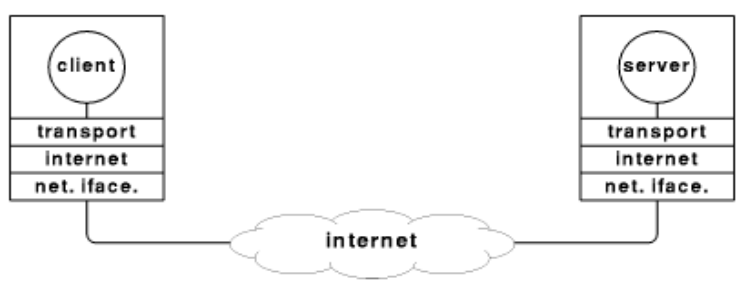
\includegraphics[width=0.7\textwidth]{./images/client-server-tcpip.png}
    \caption{
        Client \& server using TCP/IP protocols to communicate.
        Information can flow in either or both directions.
        The client \& server can interact with a transport layer protocols.
    }
\end{figure}

\subsection{Three-Tier Architecture}
A \textbf{three-tier client-server architecture} introduces a server or \textbf{agent} (or \textbf{load-balancer}) between the client \& the server.
The agent has many roles:
\begin{itemize}
    \item   Translation services: such as adapting a legacy application on a mainframe to a client-server environment.
    \item   Metering services: such as acting as a transaction monitor to limit the number of simultaneous requests to a given server.
    \item   Intelligent agent services: as in mapping a request to a number of different servers, collating the results, and returning a single response to the client.
\end{itemize}

\subsection{Network Programming Paradigms}
Practically all network programming is based on a client-server model; the only real difference in paradigms is the \textbf{level} at which the programmer operates.
The sockets API provides direct access to the available transport layer protocols.
RPC is a higher-level abstraction that hides some of the lower-level complexities.
Other approaches are also possible:
\begin{itemize}
    \item   Sockets are probably the best-known and most widely-used paradigm.
            However, problems of data incompatibility across platforms can arise.

    \item   RPC libraries aim to solve some of the basic problems with sockets and provide a level of transport independence.

    \item   Neither approach works very well with modern applications (Java RMI and other mdoern technologies, e.g., web services are better).
\end{itemize}

\section{Java RMI}
\textbf{Remote Method Invocation (RMI)} is a Java-based mechanism for distributed object computing.
RMI enables the distribution of work to other Java objects residing in other processes or on other machines.
The objects in one Java Virtual Machine (JVM) are allowed to seamlessly invoke methods on objects in a remote JVM.
To call a method of a remote object, we must first get a reference to that object, which can be obtained from  the registry name facility or by receiving the reference as an argument or return value of a method call.
Clients can call a remote object in a server that itself is a client of another server.
Parameters of method calls are passed as serialised objects: 
\begin{itemize}
    \item   types are not truncated, and therefore, object-oriented polymorphism is supported;
    \item   parameters are passed by value (deep copy) and therefore object behaviour can be passed.
\end{itemize}

The Java Object Model is still supported with distributed (remote) objects.
A reference to a remote object can be passed to or returned from local \& remote objects.
Remote object references are passed by reference: therefore, the whole object is not always downloaded.
Objects that implement the \mintinline{java}{Remote} interface are passed as a remote reference, while other objects are passed by value (using object serialisation).

\begin{figure}[H]
    \centering
    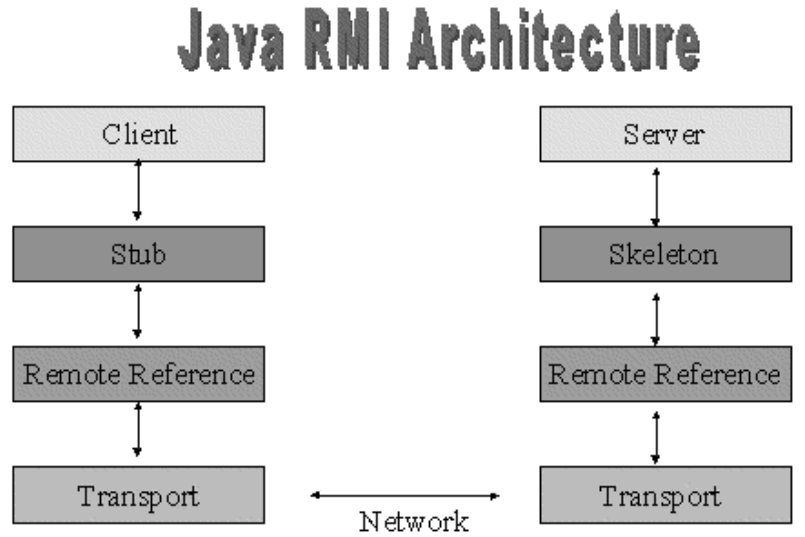
\includegraphics[width=0.8\textwidth]{./images/javarmi.png}
    \caption{Java RMI Architecture}
\end{figure}

The client obtains a reference for a remote object by calling \mintinline{java}{Naming.lookup(//URL/registered_name)} which is a method which returns a reference to another remote object.
Methods of the remote object may then be called by the client.
This call is actually to the \textbf{stub} which represents the remote object.
The stub packages the arguments (\textbf{marshalling}) into a data stream (to be sent across the network).
On the implementation side, the skeleton unmarshals the argument, calls the method, marshals the return value, and sends it back.
The stub unmarshals the return value and returns it to the caller.
The RMI layer sits on top of the JVM and this allows it to use Java Garbage Collection of remote objects, Java Security (a security manager may be set for the server, now deprecated), and Java class loading.

\subsection{Steps to Creating an RMI Application}
\begin{enumerate}
    \item   Define the interfaces to your remote objects.
    \item   Implement the remote object classes.
    \item   Write the main client \& server programs.
    \item   Create the stub \& skeleton classes by running the \textit{rmic} compiler on the remote implementation classes. (No longer needed in later Java versions).
    \item   Start the \textit{rmiregistry} (if not already started).
    \item   Start the server application.
    \item   Start the client (which contains some initial object references).
    \item   The client application/applet may then call object methods in the remote (server) program.
\end{enumerate}

\subsection{Example Java RMI Program}
\begin{code}
\begin{minted}[linenos, breaklines, frame=single]{java}
// Remote Object has a single method that is passed
// the name of a country and returns the capital city.
import java.rmi.*;

public interface CityServer extends Remote
{
    String getCapital(String Country) throws
        RemoteException;
}
\end{minted}
\caption{Example Java RMI Program}
\end{code}

\begin{code}
\begin{minted}[linenos, breaklines, frame=single]{java}
import java.rmi.*;
import java.rmi.server.*;

public class CityServerImpl
    extends UnicastRemoteObject
    implements CityServer
{
    // constructor is required in RMI
    CityServerImpl() throws RemoteException
    {
        super(); // call the parent constructor
    }

    // Remote method we are implementing!
    public String getCapital(String country) throws
        RemoteException
    {
        System.out.println("Sending return string now - country requested: " + country);
        if (country.toLowerCase().compareTo("usa") == 0)
            return "Washington";
        else if (country.toLowerCase().compareTo("ireland") == 0)
            return "Dublin";
        else if (country.toLowerCase().compareTo("france") == 0)
            return "Paris";
        return "Don't know that one!";
    }

    // main is required because the server is standalone
    public static void main(String args[])
    {
        try
        {
            // First reset our Security manager
            System.setSecurityManager(new RMISecurityManager());
            System.out.println("Security manager set");

            // Create an instance of the local object
            CityServerImpl cityServer = new CityServerImpl();
            System.out.println("Instance of City Server created");

            // Put the server object into the Registry
            Naming.rebind("Capitals", cityServer);
            System.out.println("Name rebind completed");
            System.out.println("Server ready for requests!");
        } catch(Exception exc)
        {
            System.out.println("Error in main - " + exc.toString());
        }
    }
}
\end{minted}
\caption{Example Server Implementation}
\end{code}

\begin{code}
\begin{minted}[linenos, breaklines, frame=single]{java}
public class CityClient
{
    public static void main (String args[])
    {
        CityServer cities = (CityServer) Naming.lookup("//localhost/Capitals");
        try {
            String capital = cities.getCapital("USA");
            System.out.println(capital);
        } catch (Exception e) {}
    }
}
\end{minted}
\caption{Example Client Implementation}
\end{code}

No distributed system can mask communication failures: method semantics should include failure possibilities.
Every RMI remote method must declare the exception \mintinline{java}{RemoteException} in its \mintinline{java}{throw} clause.
This exception is thrown when method invocation or return fails.
The Java compiler requires the failures to be handled.
\\\\
When implementing a remote object, the implementation class usually extends the RMI class \mintinline{java}{UnicastRemoteObject}: this indicates that the implementation class is used to create a single (non-replicated) remote object that uses RMI's default sockets-based transport for communication.
If you choose to extend a remote object from a non-remote class, you need to explicitly export the remote object by calling the method \mintinline{java}{UnicastRemoteObject.exportObject()}.
\\\\
The main method of the service first needs to create \& install a \textbf{security manager}, either the \mintinline{java}{RMISecurityManager} or one that you have defined yourself.
A security manager needs to be running so that it can guarantee that the classes loaded do not perform ``sensitive'' operations.
If no security manager is specified, no class loading for RMI classes is allowed, local or otherwise.
\\\\
TO make classes available via a web server (or your classpath), copy them into your public HTML directory.
Alternatively, you could have compiled your files directly into your public HTML directory:
\begin{minted}[linenos, breaklines, frame=single]{shell}
javac -d ~/project_dir/public_html City*.java
rmic -d ~/project_dir/public_html  CityServerImpl
\end{minted}

The files generated by \mintinline{shell}{rmic} (in this case) are: \verb|CityServerImpl_Stub.class| \& \verb|CityServerImpl_Skel.class|.
\\\\
\textbf{Polymorphic distributed computing} is the ability to recognise (at runtime) the actual implementation type of a particular interface.
We will use the example of a remote object that is used to computer arbitrary tasks:
\begin{itemize}
    \item   Client sends task object to compute server.
    \item   Compute server runs task and returns result.
    \item   RMI loads task code dynamically in the server.
\end{itemize}
This example shows polymorphism on the server, but it also works on the client, for example the server returns a particular interface implementation.
\\\\
Our example task will be a simple interface that defines an arbitrary task to compute:
\begin{code}
\begin{minted}[linenos, breaklines, frame=single]{java}
public interface Task extends Serializable
{
    Object run();
}
\end{minted}
\caption{Simple \mintinline{java}{Task} interface}
\end{code}

We will also define a \mintinline{java}{Remote} interface:
\begin{code}
\begin{minted}[linenos, breaklines, frame=single]{java}
import java.rmi.*;

public interface Compute extends Remote
{
    Object runTask(Task t) throws RemoteException;
}
\end{minted}
\caption{Simple \mintinline{java}{Task} interface}
\end{code}

A task may create a \mintinline{java}{Remote} object on the server and return a reference to that object; the \mintinline{java}{Remote} object will be garbage-collected when the returned reference is dropped (assuming that no-one else is given a copy of the reference).
A task may create a \mintinline{java}{Serializable} object and return a copy of that object; the original object will be locally garbage-collected when the \mintinline{java}{Task} ends.
If the \mintinline{java}{Task} creates an object that is neither a \mintinline{java}{Remote} nor a \mintinline{java}{Serializable} object, a marshalling exception will be thrown.

\begin{code}
\begin{minted}[linenos, breaklines, frame=single]{java}
import java.rmi.*;
import java.rmi.server.*;

public class ComputeServer extends UnicastRemoteObject implements Compute
{
    public ComputeServer() throws RemoteException {}

    public Object runTask(Task t)
    {
        return t.run();
    }
}
\end{minted}
\caption{Compute server implementation}
\end{code}

\begin{code}
\begin{minted}[linenos, breaklines, frame=single]{java}
public static void main(String args[])
{
    System.setSecurityManager(new RMISecurityManager());
    try
    {
        ComputeServer cs = new ComputeServer();
        Naming.rebind("Computer", cs);
    }
    catch (Exception e)
    {
        // Exception handling
    }
}
\end{minted}
\caption{Compute server implementation}
\end{code}

\begin{code}
\begin{minted}[linenos, breaklines, frame=single]{java}
public class Pi implements Task
{
    private int places;

    public Pi (int places)
    {
        this.places = places;
    }

    public Object run()
    {
        // Compute Pi
        return result;
    }
}
\end{minted}
\caption{Task to compute $\pi$}
\end{code}

\begin{code}
\begin{minted}[linenos, breaklines, frame=single]{java}
Compute comp = (Compute) Naming.Lookup("//www.t.nuigalway.ie/Computer");

Pi pi = new Pi(100);
Object piResult = comp.runTask(pi);

// print results
\end{minted}
\caption{The client}
\end{code}

In conclusion, RMI is flexible and allows us to pass objects (both \mintinline{java}{Remote} \& \mintinline{java}{Serializable}) by exact type rather than declared type and download code to introduce extended functionality in both client \& server.
However, it is Java-only and has been superseded by SOAP \& REST as the de-facto standards for communicating with remote services.
Nonetheless, RMI is still worth  learning to help understand concepts around distributed objects \& distributed systems architecture. 

\section{Enterprise Java Beans}
\subsection{Distributed System Scenario}
Imagine a worldwide financial company with 10,000 online customers that wants to add a new currency converter software component that is heavily used with 1,0000 hits/second.
The design will consist of the business logic and the distributed infrastructure.
The distributed infrastructure includes security, load-balancing, transaction management, \& object-relational mapping; Enterprise Java Beans takes care of this, and provides an API \& framework.

\begin{figure}[H]
    \centering
    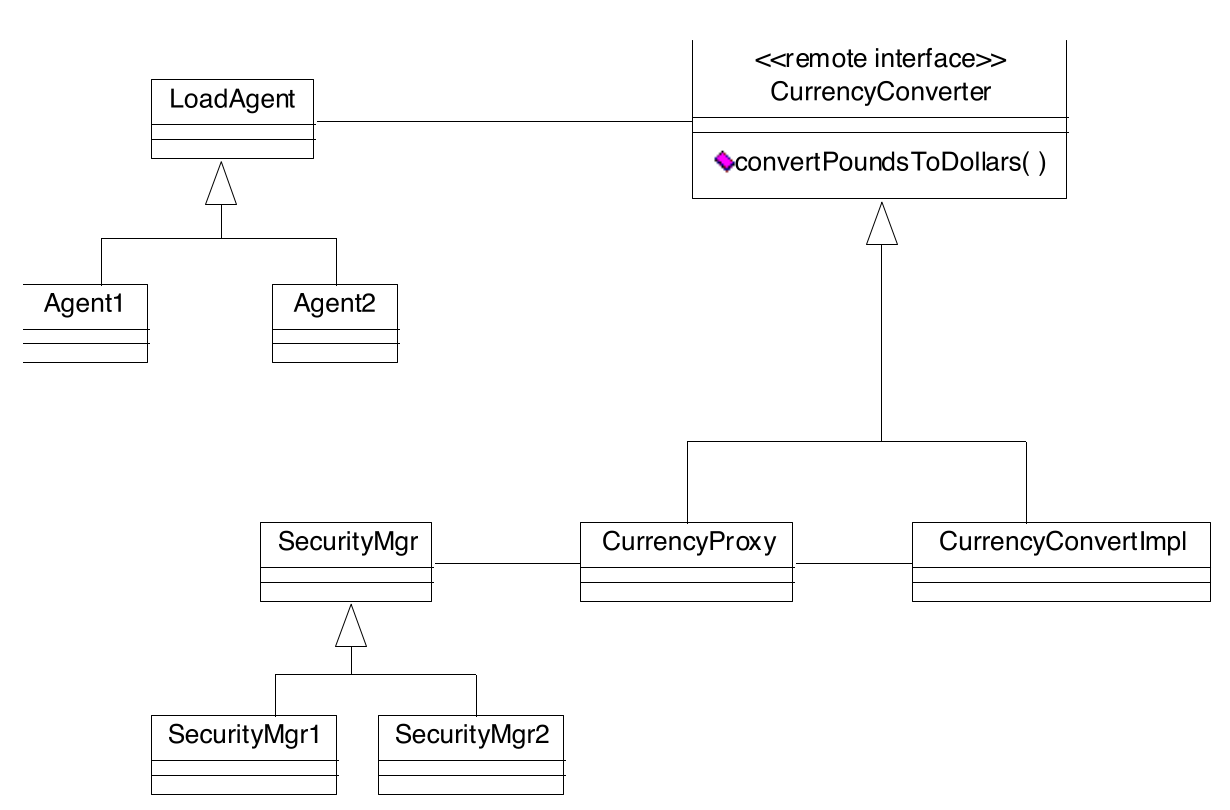
\includegraphics[width=0.7\textwidth]{./images/distributed_system_scenario.png}
    \caption{
        Business logic, distribute the object, add security manager, add load balancing agent.
    }
\end{figure}

\subsection{EJB}
\textbf{Enterprise Java Beans (EJB)} is a server-side component architecture that enables and simplifies the process of building enterprise-class distributed object applications in Java.
It allows you to write scalable, reliable, and secure applications without writing your own complex distributed object frameworks.
EJB is a \textit{specification}.

\begin{figure}[H]
    \centering
    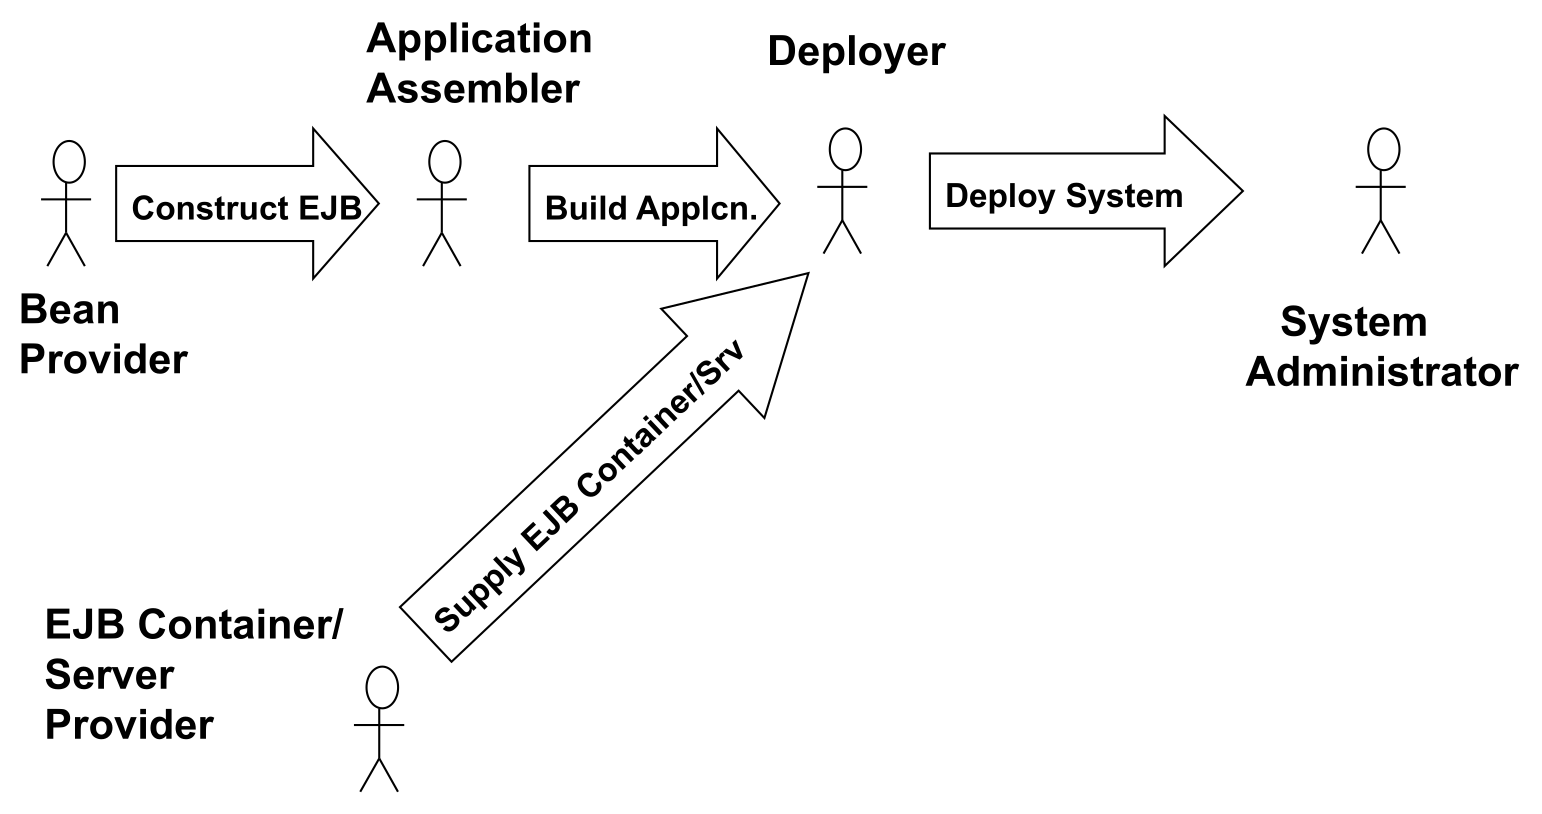
\includegraphics[width=0.7\textwidth]{./images/the_ejb_proces.png}
    \caption{
        The EJB process
    }
\end{figure}

The \textbf{EJB Container} is where the EJBs run and is responsible for managing EJBs.
The \textbf{EJB Server} is a runtime environment for container(s) that manages the low-level system resources.

\begin{figure}[H]
    \centering
    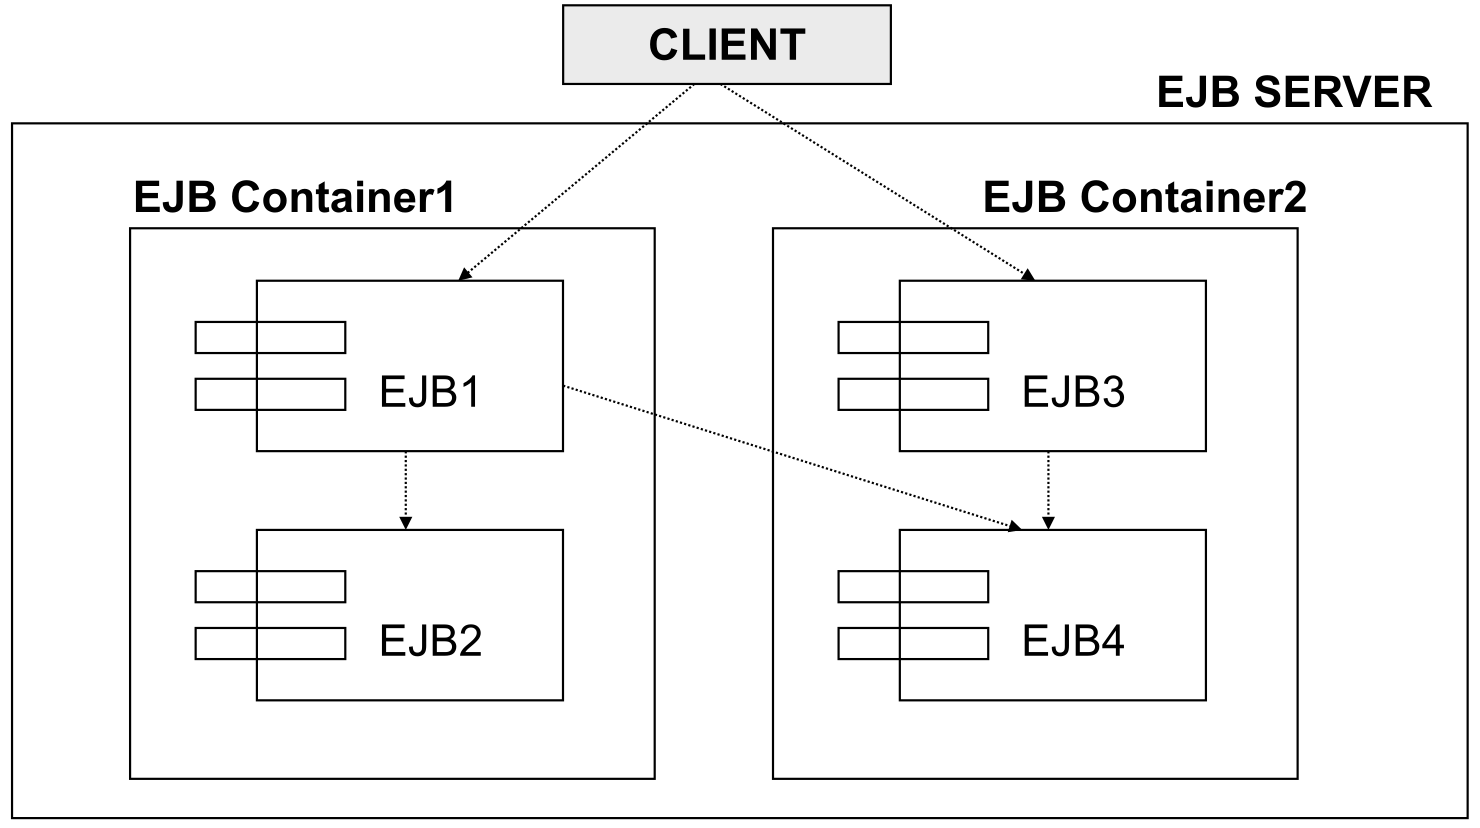
\includegraphics[width=0.7\textwidth]{./images/ejb_server_and_container.png}
    \caption{ The EJB server \& containers }
\end{figure}

\begin{figure}[H]
    \centering
    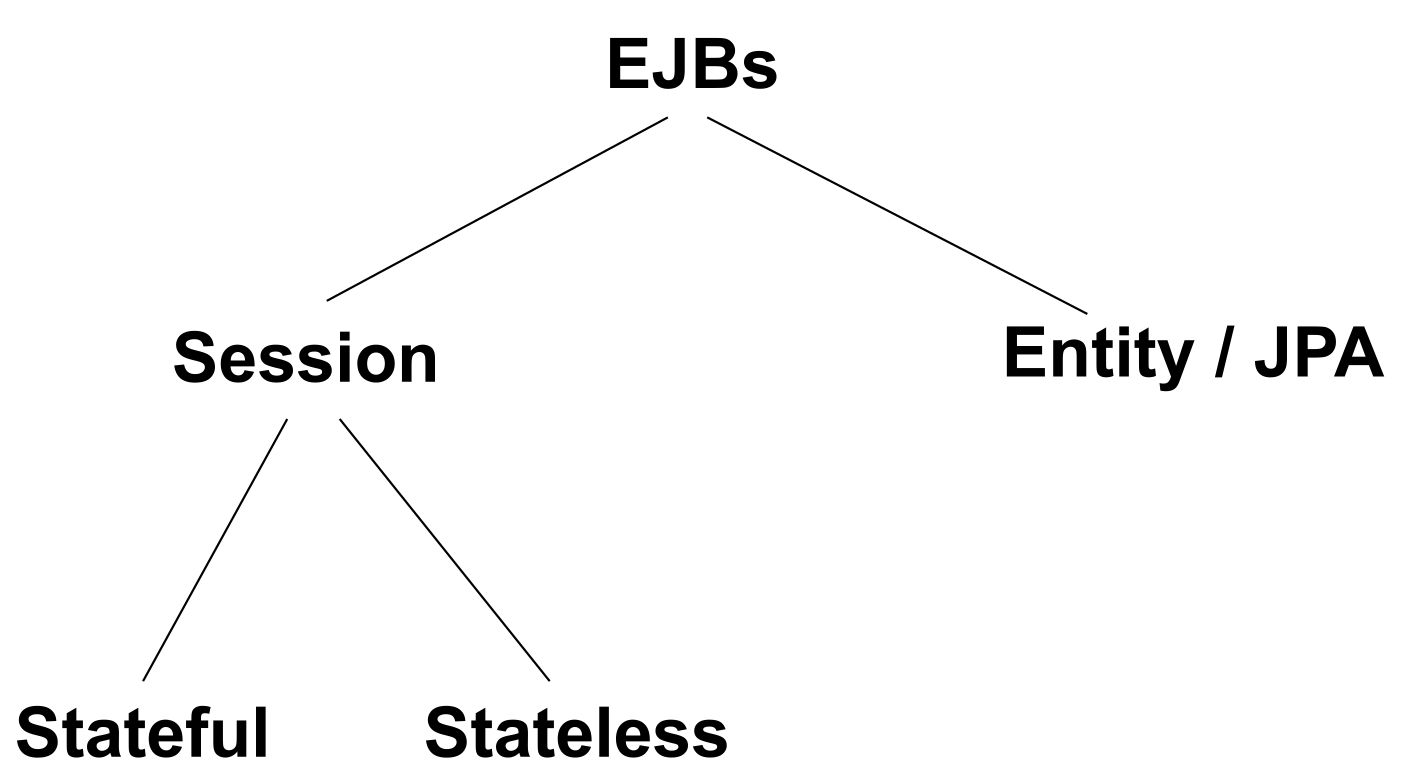
\includegraphics[width=0.7\textwidth]{./images/ejb_bean_types.png}
    \caption{ EJ Bean types }
\end{figure}

\textbf{Session beans} are ``business process objects'' (e.g., price quoting, order entry, video compression, stock trades, etc.) and live for as long as the client's session.
They are usable by 1 client at a time and are \textit{not} shared.
The EJB server manages the lifetime of beans.
\textbf{Stateless session beans} are single request with no state kept, e.g., currency converter, compression utility, or credit card verification.
\\\\
\textbf{Entity beans / JPA} represent persistent data.
They are the object-oriented in-memory view of data in an underlying data store.
They are long-lasting and have shared access.
Sub-types of entity beans include: bean-managed persisted entity beans and container-manager persistent entity beans.
\textbf{Bean-managed persistence} must be persisted manually and must look after saving, loading, \& finding.
They make use of a persistence API such as JDBC or SQL/J.
\textbf{Container-managed persistence} is automatic persistence wherein the container/server looks after the loading, saving, \& finding of component data.
You must describe what you want persisted.
Deployment tools provide support for defining simple object-relational mappings.
\\\\
The client never invokes the bean instance, instead it invokes the \textbf{EJB object} by an invocation that is intercepted by the container, delegated to the bean instance.
The EJB object is a surrogate, network-aware wrapper object that serves as a layer of indirection between the client \& the bean; it is essentially the glue between the client \& the bean.
EJB objects must clone every business method that your bean class exposes, specified in the remote interface.
All remote interfaces derive from \mintinline{java}{javax.ejb.EJBObject}.

\begin{figure}[H]
    \centering
    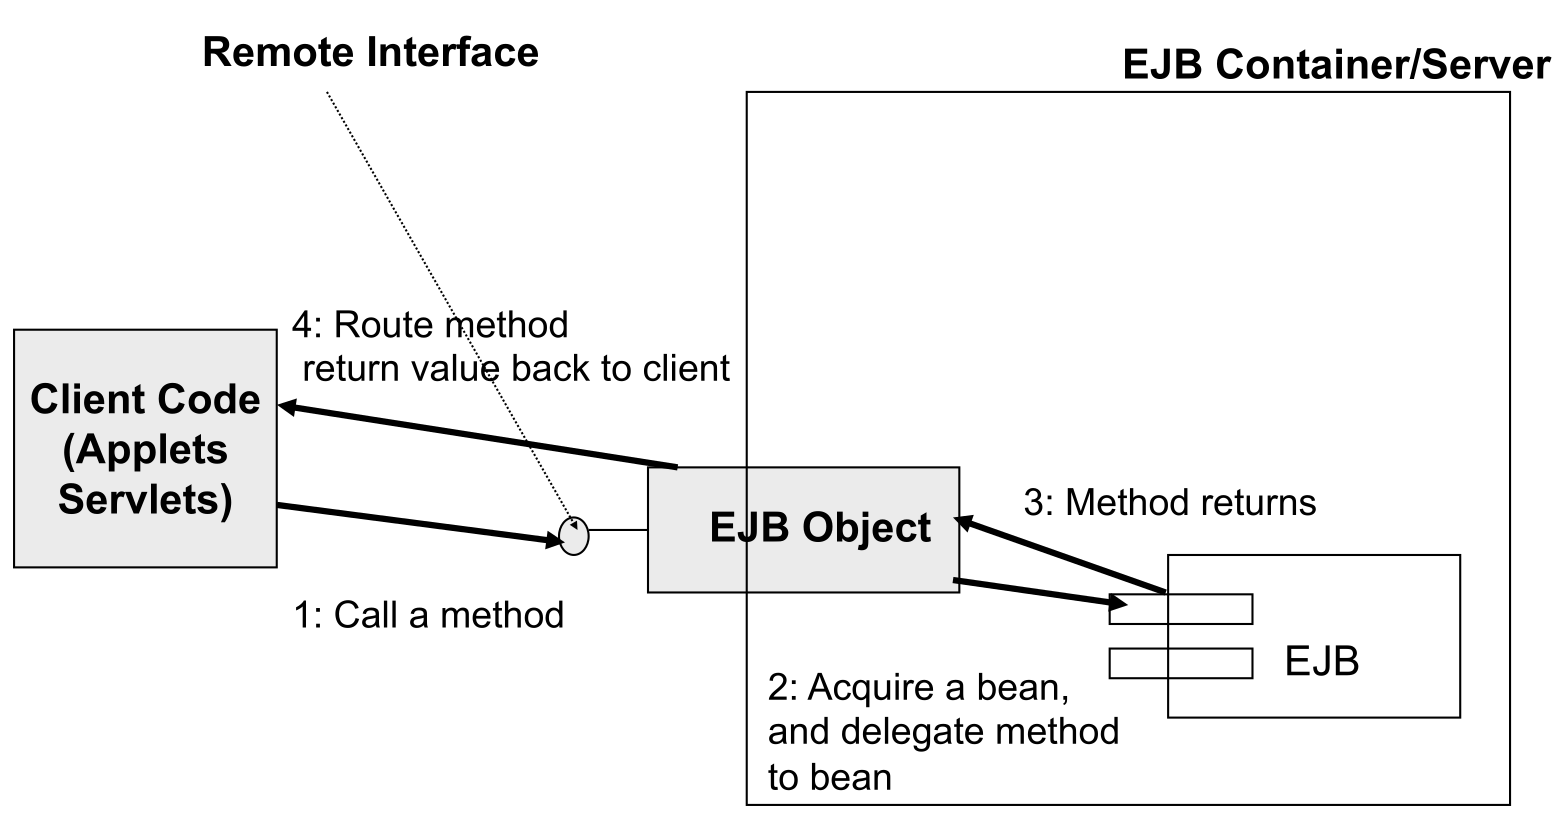
\includegraphics[width=0.7\textwidth]{./images/ejb_objets.png}
    \caption{ EJB Objects }
\end{figure}

The \textbf{session bean interface} is implemented by all session beans and specifies lifecycle methods that may be implemented inn the bean such as \mintinline{java}{setSessionContext}, \mintinline{java}{ejbCreate}, \mintinline{java}{ejbRemove}, \mintinline{java}{ejbPassivate}, \& \mintinline{java}{ejbActivate}.
\\\\
The \textbf{Java Naming \& Directory Interface} is used to find an object.
The resource (e.g., a bean) is associated with a nickname when deploying; clients of this bean can then use this nickname to look up the resource across a deployment.
The client code looks up the reference in JNDI and calls business methods on the EJB object.

\subsubsection{Entity EJBs}
\textbf{Entity EJBs} are object-based representations of information-tier data such as data stored in a relational database.
They represent a particular unit of data, e.g., a record in a database.
There are two types of entity EJB:
\begin{itemize}
    \item   Bean-managed persistence;
    \item   Container-managed persistence.
\end{itemize}





\end{document}
